%\IfFileExists{ajr.sty}
\documentclass[12pt,a5paper]{article}
%{\documentclass[12pt,a5paper]{refart}}
%\IfFileExists{ajr.sty}{\usepackage{ajr}}{}
\usepackage[margin=6mm,bottom=15mm]{geometry}
\usepackage{amsmath,defns,reducecode}
\usepackage{ProTex}
\AlProTex{blue,<<<>>>,title,list,`}
\usepackage{euler,natbib,amsmath}
\usepackage{url}
\usepackage{graphicx}
\usepackage{hyperref} 
\hypersetup{pdftex,
            backref=true,
            hyperindex=true,
            colorlinks=true,
            citecolor=blue,
            bookmarks=true,
            breaklinks=true}

\allowdisplaybreaks

\newcommand{\zs}{\zeta}
\newcommand{\uu}{{\bar u}}
\newcommand{\vv}{{\bar v}}
\newcommand{\bq}{{\bar q}}
\newcommand{\qq}{{\bar{\vec q}}}
\newcommand{\ee}{\textsc{e}}
\newcommand{\rnu}{R_\nu}
\newcommand{\ros}{{\dot\varepsilon}}



\title{Modelling 3D turbulent floods based upon the Smagorinski large eddy closure}

\author{Meng Cao\thanks{School of Mathematical Sciences,
University of Adelaide, South Australia 5005.  \protect\url{mailto:anthony.roberts@adelaide.edu.au}}
\qquad 
A.~J. Roberts\thanks{School of Mathematical Sciences,
University of Adelaide, South Australia 5005.  \protect\url{mailto:meng.cao@adelaide.edu.au}}}

%\date{31 May 2012}

\begin{document}
    
\maketitle

\section*{Abstract}

Rivers, floods and tsunamis are often very turbulent. Conventional models of such environmental fluids are typically based on depth-averaged inviscid irrotational flow equations. We explore changing such a base to the turbulent Smagorinski large eddy closure. The aim is to more appropriately model the fluid dynamics of such complex environmental fluids by using such a turbulent closure. Large changes in fluid depth are allowed. Computer algebra constructs the slow manifold of the flow in terms of the fluid depth~$h$ and the mean turbulent lateral velocities~$\bar u$ and~$\bar v$. The major challenge is to deal with the nonlinear stress tensor in the Smagorinski closure. The model integrates the effects of inertia, self-advection, bed drag, gravitational forcing and turbulent dissipation with minimal assumptions. Although the resultant model is close to established models, the real outcome is creating a sound basis for the modelling so others, in their modelling of more complex situations, can systematically include more complex physical processes.

\paragraph{Keywords} turbulent flood, tsunami, Smagorinski closure, channel flows

\tableofcontents

\section{Intoduction}

Environmental turbulent fluids have large wave length compared with the fluid depth. Large eddy viscosity model is always used to account for the turbulence. Compound channel flows, as a typical of such environmental turbulent fluid, are investigated experimentally and numerically~\cite[e.g.]{Bousmar2002,Liu2009,Demuren1993}. Conventional models of such flows are carried out by depth-averaging the flow equations. \cite{Bousmar2002} proposed an exchange discharge model~(\textsc{edm}) by depth-averaging the Navier-Stokes equations. The~\textsc{edm} solves the momentum transfers experimentally and numerically due to the turbulent exchange and geometrical transfer between channel subsections, the channel and the shallow regions. The~\textsc{edm} predicts the discharge and water profile computation successfully and supports our numerical analysis in Section~\ref{sec-straight}. \cite{Liu2009} simulated shallow water flows in curved and meandering channels by a depth-averaged lattice Boltzmann model with adding the large eddy simulation model to account for turbulence. The results of~\cite{Liu2009} will be compared with our simulations in the Section~\ref{sec-meander}. 

However, these kinds of depth-averaging models are conjectured to be deficient by~\cite{Roberts1996}, since depth-averaging is qualitatively unsound except perhaps for low Reynolds number flows. Instead of depth-averaging flow equations, Section~\ref{low-order} resolves the turbulent dynamics based on the centre manifold theory, which assures there existing a slow manifold for the evolution of the continuity equation~\eqref{eq:cont}, momentum equation~\eqref{eq:mom} and nonlinear shear tensor in the Smagorinski closure~\eqref{eq:stress}.
Section~\ref{sec-straight} and~\ref{sec-meander} use the resulting model simulate the flows over straight and meandering compound channels and compares with the published data~\cite[e.g.]{Bousmar2002,Liu2009}.


\section{Description of the turbulence model}
\label{description}

\paragraph{Governing differential equations} Assume three dimensional incompressible and irrotational turbulent fluid flowing down a slightly sloping ground. Define the Cartesian coordinates with the lateral directions~$x_1=x, x_2=y$ and the normal direction~$x_3=z$. Let the turbulent fluid have thickness~$h(x,y,t)$ over the ground~$b(x,y)$ with a slope~$\theta$, turbulent mean velocity field~$\bar q=(u,v,w)=(u_1,u_2,u_3)$, and turbulent mean pressure field~$p$. Nondimensionalising the defined variables with respect to some velocity scale, typical fluid thickness and fluid density, the nondimensional governing partial differential equations for the incompressible, irrotational, three dimensional, turbulent mean fluid are the continuity equation
\begin{equation}
    \divv\vec q=\D xu+\D yv+\D zw=0\,,\label{eq:cont}
\end{equation}
and the momentum equation
\begin{equation}
    \D t{\vec q} +\vec q\cdot\grad\vec q
    =-\grad p +\divv\vec\tau +\vec{g}\,,\label{eq:mom}
\end{equation}
where~$\tau$ is the turbulent mean stress tensor and~$\vec g=(g_1,0,g_3)$ is the nondimensional forcing from gravity.

\paragraph{Smagorinski large eddy closure} The effects of turbulence are modelled by the eddy viscosity~$\nu$, which is related to the mean shear stress through the equation of
\begin{equation}
\tau_{ij}=2\nu\ros_{ij}\,,\label{eq:tau}
\end{equation}
with the indexes~$i,j=1,2,3$ indicating in the~$x, y$ and~$z$ directions. Define the turbulent mean strain-rate tensor~\cite[e.g.]{Roberts2008,Georgiev2008}
\begin{equation}
	\ros_{ij} =\frac12\left( \D{x_j}{u_i} +\D{x_i}{u_j}\right) \,,\label{eq:strainrate}
\end{equation}
and then the turbulent mean stress tensor for the turbulent fluid is
\begin{equation}
\sigma_{ij}=-p\delta_{ij}+2\rho\nu\ros_{ij}\,.\label{eq:sigma}
\end{equation}
When the eddy viscosity~$\nu$ is constant, equation~\eqref{eq:sigma} models a Newtonian fluid. In the Smagorinski model~\cite[e.g.]{Ozgokmen2007a}, the eddy viscosity~$\nu$ varies linearly with the magnitude~$\ros$ of the second invariant of the strain-rate tensor,
\begin{equation}
  \nu=c_th^2\ros\quad\text{where}\quad |\ros|^2=\sum_{i,j}\ros_{ij}^2\,.\label{eq:nu}
\end{equation}
\cite{Roberts2008} considered the proportionality~$c_t\approx0.02$ for the turbulent environmental flows by comparison with established channel flow experiments~\cite[e.g.]{Nezu2005}. Thus, the equations~\eqref{eq:tau}$-$\eqref{eq:nu} give the turbulent mean stress tensor
\begin{equation}
\tau_{ij}=2\nu(\ros)\ros_{ij}=c_th^2\ros\left( \D{x_j}{u_i} +\D{x_i}{u_j}\right) \,.\label{eq:stress}
\end{equation}

\paragraph{Boundary conditions} Formulate boundary conditions on the ground~$b(x,y)$ and free surface~$\eta(x,y,t)=h(x,y,t)+b(x,y)$ in terms of the turbulent mean velocity field~$\vec q(x,y,t)$ and the fluid depth~$h(x,y,t)$. On the ground, no flow penetrating the ground indicates~$\vec q\cdot\vec n=0$, that is,
\begin{equation}
w=ub_x+vb_y\ \text{on}\ z=b\,,
\label{eq:nopen}
\end{equation}
where the vector
\begin{equation}
\vec n=\frac{1}{\sqrt{1+b_x^2+b_y^2}}(-b_x,-b_y,1)\,,\label{eq:vecn}
\end{equation} 
presents the unit vector normal to the ground.  
\\
Putting a slip law on the ground to account for a relatively thin turbulent boundary layer, 
\begin{equation}
\vec q_{\text{tan}}=c_uh\frac{\partial\vec q_{\text{tan}}}{\partial\vec n}\,\ \text{on}\ z=b\,,
\label{bc:slip}
\end{equation} 
where the term~$\vec q_{\text{tan}}$ represents the velocity tangential to the ground. \cite{Roberts2008} consider the constant~$c_u\approx1.85$ to match open channel flow observations. In applications, the coefficient~$c_u$ would change for different ground roughness. To detail the boundary condition~\eqref{bc:slip}, assume
\begin{align*}&
\vec t_x=\frac{1}{\sqrt{1+b_x^2}}(1,0,b_x)\,,
\\&
\vec t_y=\frac{1}{\sqrt{1+b_y^2}}(0,1,b_y)\,,
\end{align*}
are unit vectors tangential to the ground in the~$x$ and~$y$ directions. For simplicity, consider
\begin{equation*}
\vec q_{\text{tan}}=(\vec t_x\cdot\vec q)\vec t_x+(\vec t_y\cdot\vec q)\vec t_y\,.
\end{equation*}
Thus, the boundary condition~\eqref{bc:slip} becomes
\begin{eqnarray*}
&&\vec t_x\cdot\vec q_{\text{tan}}=c_uh\frac{\partial}{\partial\vec n}(\vec t_x\cdot\vec q_{\text{tan}})\,\ \text{on}\ z=b\,,\\
&&\vec t_y\cdot\vec q_{\text{tan}}=c_uh\frac{\partial}{\partial\vec n}(\vec t_y\cdot\vec q_{\text{tan}})\,\ \text{on}\ z=b\,,
\end{eqnarray*}
which are
\begin{align}&
\frac{1}{\sqrt{1+b_x^2}}(u+wb_x)=\frac{c_uh}{\sqrt{1+b_x^2+b_y^2}}\frac{\partial}{\partial\vec n}(u+wb_x)\ \text{on}\ z=b\,,\label{slip:u}\\&
\frac{1}{\sqrt{1+b_y^2}}(v+wb_y)=\frac{c_uh}{\sqrt{1+b_x^2+b_y^2}}\frac{\partial}{\partial\vec n}(v+wb_y)\ \text{on}\ z=b\,.\label{slip:v}
\end{align}
\\
On the free surface, the kinematic condition is 
\begin{equation}
 \frac{\partial\eta}{\partial t}+u\frac{\partial\eta}{\partial x}+v\frac{\partial\eta}{\partial y}=w\quad\text{on}\quad z=\eta\,,
\end{equation}
where the term~$\eta=h+b$ denotes the turbulent mean location of the free surface. Assume the pressure of the air on the free surface is zero. Thus the turbulent mean stress normal to the free surface is also zero,
\begin{equation}
    -p+\frac{\tau_{33} -2\eta_x\tau_{13} -2\eta_y\tau_{23}
    +\eta_x^2\tau_{11} +2\eta_x\eta_y\tau_{12}+\eta_y^2\tau_{22}}
    {1+\eta_x^2+\eta_y^2}
     =0 \ \text{on }
    z=\eta\,.
    \label{bc:ttz}
\end{equation}
There must be no turbulent mean, tangential stress at the free surface,
\begin{eqnarray}&&
    (1-\eta_x^2)\tau_{13}+\eta_x(\tau_{33}-\tau_{11})-\eta_y(\tau_{12}+\eta_x\tau_{23})=0
    \quad\text{on } z=\eta\,,
    \label{bc:ttx} \\&&
    (1-\eta_y^2)\tau_{23}+\eta_y(\tau_{33}-\tau_{22})
    -\eta_x(\tau_{12}+\eta_y\tau_{13})=0
    \quad\text{on}\ z=\eta\,.
    \label{bc:tty}
\end{eqnarray}




\section{Low order models of the dynamics}
\label{low-order}

This section focusses on interpreting the application of centre manifold theory and the resulting low order models.

Instead of depth-averaging equations, we apply the centre manifold theory to deal with the turbulent dynamics across the fluid layer. \cite{Roberts2008,Georgiev2008} detailed similar approaches by introducing a parameter~$\gamma$ to the boundary conditions~\eqref{bc:ttx} and~\eqref{bc:tty}, where~$\gamma=0$ provides analytic analysis and~$\gamma=1$ recovers the physical case. Centre manifold theory assures that there exist a slow manifold for the evolution of equations~\eqref{eq:cont},~\eqref{eq:mom} and~\eqref{eq:stress}.
 
\cite{Roberts:2008fk} described the algebra of constructing the existed slow manifold. Developed computer algebra program derives the evolutions of the depth field $h(x,y,t)$ and the mean lateral velocities~$\bar u(x,y,t)$ and~$\bar v(x,y,t)$ in the~$x$ and~$y$ directions. The evolution of~$h(x,y,t)$, $\bar u(x,y,t)$ and~$\bar v(x,y,t)$ are described by the conservation equation and momentum equations,
\begin{align}
\frac{\partial h}{\partial t}&
\approx-\frac{\partial h\bar u}{\partial x}-\frac{\partial h\bar v}{\partial y}\,,\label{smag:h}
\\
\frac{\partial\bar u}{\partial t}&
\approx-0.00293\gamma\frac{\bar u\sqrt{\bar u^2+\bar v^2}}{h}+0.985g_x+0.00799\gamma g_x
\nonumber\\&
-0.985g_z\left(\frac{\partial h}{\partial x}+\frac{\partial b}{\partial x}\right)-0.00799\gamma g_z\D xb
-0.00799\gamma g_z\D xh
\nonumber\\&
-1.03\bar v\frac{\partial\bar u}{\partial y}-1.045\bar u\frac{\partial\bar u}{\partial x}-0.0115\uu\D{y}{\vv}
\nonumber\\&
+0.0136\gamma\vv\D{y}{\uu}+0.00305\gamma\uu\D{y}{\vv}+0.0204\gamma\uu\D{x}{\uu}
\nonumber\\&
+0.0194h\sqrt{\uu^2+\vv^2}\D x\vv\D y\vv-0.00784\frac{h\uu\vv}{\sqrt{\uu^2+\vv^2}}\DD{y}{\vv}
\nonumber\\&
+0.00119\frac{h\uu\vv}{\sqrt{\uu^2+\vv^2}}\DD x\vv-0.251\frac{h\uu^2}{\sqrt{\uu^2+\vv^2}}\D x\vv\D y\vv
\nonumber\\&
+0.237h\sqrt{\uu^2+\vv^2}\DD y\uu+0.698\frac{h\uu\vv}{\sqrt{\uu^2+\vv^2}}\D x\uu\D y\uu
\nonumber\\&
+0.0266h\sqrt{\uu^2+\vv^2}\DD x\uu+0.468\frac{h\uu^2}{\sqrt{\uu^2+\vv^2}}\DD x\uu\,,
\label{smag:u}
\\
\frac{\partial\bar v}{\partial t}&
\approx-0.00293\gamma\frac{\bar v\sqrt{\bar u^2+\bar v^2}}{h}
\nonumber\\&
-0.989g_z\left(\frac{\partial h}{\partial y}+\frac{\partial b}{\partial y}\right)
-0.00366\gamma g_z\D yh-0.00366\gamma g_z\D yb
\nonumber\\&
-1.042\bar v\frac{\partial\bar v}{\partial y}-1.026\bar u\frac{\partial\bar v}{\partial x}
+0.00371\uu\D y\uu-0.0152\vv\D x\uu
\nonumber\\&
+0.0167\gamma\vv\D y\vv+0.00975\gamma\uu\D x\vv-0.0038\gamma\uu\D y\uu+0.00686\gamma\vv\D x\uu
\nonumber\\&
+0.2488h\sqrt{\uu^2+\vv^2}\DD y\vv+0.00606h\sqrt{\uu^2+\vv^2}\DD x\vv
\nonumber\\&
+0.213\frac{h\uu\vv}{\sqrt{\uu^2+\vv^2}}\D x\vv\D y\vv-0.0119\frac{h\uu^2}{\sqrt{\uu^2+\vv^2}}\DD x\vv
\nonumber\\&
-0.243\frac{h\uu\vv}{\sqrt{\uu^2+\vv^2}}\DD y\uu+0.256h\sqrt{\uu^2+\vv^2}\D x\uu\D y\uu
\nonumber\\&
-0.72\frac{h\uu^2}{\sqrt{\uu^2+\vv^2}}\D x\uu\D y\uu+0.235\frac{h\uu\vv}{\sqrt{\uu^2+\vv^2}}\DD x\uu
\,,\label{smag:v}
\end{align}
The equations~\eqref{smag:h}$-$\eqref{smag:v} come as a result of taking into account the relatively slow variations in the lateral directions~$x$ and~$y$, and small but non-zero~$\partial_x$ and~$\partial_y$, thus these equations are smooth and slow in~$x$ and~$y$.  The momentum equations~\eqref{smag:u} and~\eqref{smag:v} incorporate the inertial terms~$\bq_t$, self-advection terms~$\bq\frac{\partial x}{\partial\bq}$, bed drag terms~$\bq\sqrt{\uu^2+\vv^2}/h$, gravitational forcing~$g_x-g_z\frac{\partial(h+b)}{\partial x_i}$, and other terms related to the turbulent mixing, where~$\bq=(\uu,\vv)$ and~$i=1,3$. Note that although the equations~\eqref{smag:h}$-$\eqref{smag:v} are expressed by the depth averaged lateral velocities, they are derived not by depth-averaging, but instead by systematically accounting for interaction between vertical profiles of velocitiy/stress and bed drag and lateral space variations. The coefficients in equations~\eqref{smag:h}$-$\eqref{smag:v} are supported by centre manifold theory. When the parameter~$\gamma=1$, the model would describe the physical dynamics.


\section{Modelling flows over straight channels}
\label{sec-straight}

\begin{figure}
\centering
\begin{tabular}{c@{}c}
\rotatebox{90}{\hspace{9ex}channel depth} &
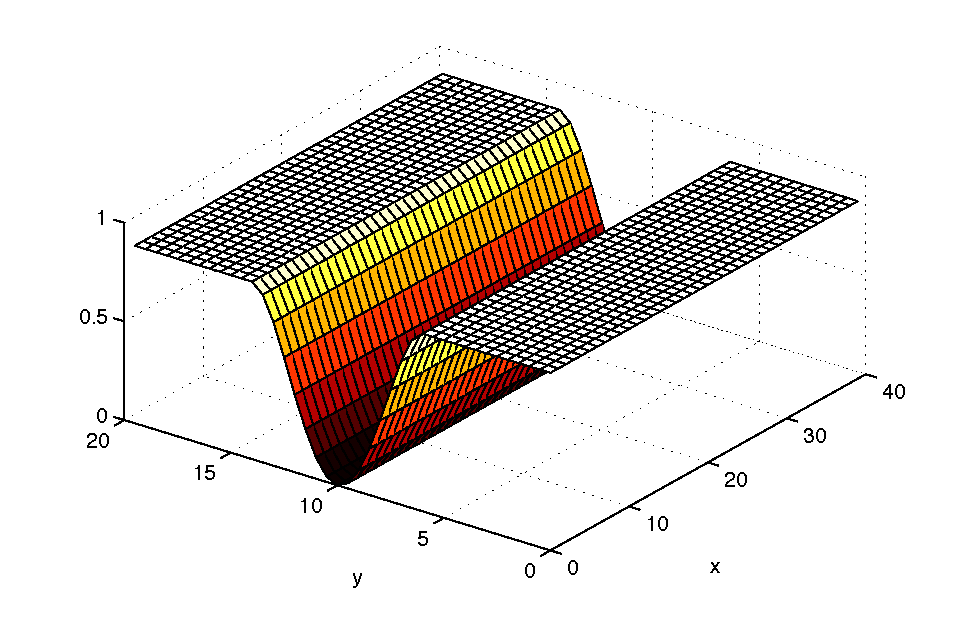
\includegraphics[width=0.7\textwidth]{straight-channel}
\end{tabular}
\caption{Schematic straight open channel. The channel locates at~$y=10$. The width and the maximum depth of the channel are~$8$ and~$0.9$, respectively. The slope of the channel in the~$x$ direction is~$\theta=0.01$. Assume the still water level is~$1$, and thus the depth of the shallow regions is~$0.1$.}
\label{straight-channel}
\end{figure}%

This section focuses on the application of the resulting model for turbulence flow over straight open channels. Consider the turbulence flow over a slightly sloping ground with an open channel, shown in Figure~\ref{straight-channel}. Compare this channel flow with viscous film flow on a substrate with a small channel by~\cite{Robertsli2006} and the experiments of~\cite{Bousmar2002,Bousmar2003a} for turbulent flow over flood plains and channels in a flume with water of variable depth.
 
 Let~$x$ be the along stream coordinate,~$y$ be the horizontal distance across the stream on the channel and~$z$ be normal to the channel. Consider the water of a depth~$h(x,y,t)$ flows with the mean lateral velocities~$\bar u(x,y,t)$ and~$\bar v(x,y,t)$ along the channel of
\begin{equation}
b(x,y)=B\left\{1-\left[1-\left(\frac{y-\alpha}{\beta}\right)^2\right]^2\right\}\,,\label{bed:straight}
\end{equation}
where~$\alpha$ and~$\beta$ denote the location and width of the channel, and~$B$ is the mid-depth of the channel. Figure~\ref{straight-channel} describes the scaled open channel located at~$y=\alpha=10$ and with the width~$2\beta=8$. The slope of the channel in the~$x$ direction is~$\theta=0.01$. Consider the initial still water level is~$1$. The mid-depth of the channel is~$B=0.9$ and then the depth of the shallow regions is~$1-B=0.1$.
The channel of~\cite{Bousmar2002} is about two times as deep in the constant channel as in the flood plain.

Consider the fluid of a scaled initial level~$h(x,y,t)+b(x,y)=1$ flowing with small mean lateral velocity~$\uu(x,y,t)$ down the open channel shown in Figure~\ref{straight-channel}. Nondimensionalise the variables of fluid depth~$h(x,y,t)$ and mean lateral velocities~$\uu(x,y,t)$ and~$\vv(x,y,t)$ with respect to some velocity scale, a typical depth and a fluid density, and consider~$g=1$. Equations~\eqref{smag:h}$-$\eqref{smag:v} describe the dynamics of this fluid with the periodic boundary conditions both in the~$x$ and~$y$ directions for both the flow and channel. Figure~\ref{straight-v-history} shows the history of the mean velocity~$\sqrt{\uu^2+\vv^2}$ until the time~$t=400$. The relevant parameters are defined in Figure~\ref{straight-channel}. The zero slopes of the curves after time~$t=200$ certify that the fluid converges to steady state. The ripples on the curves demonstrate small roll waves occurring on the free surface. 

Figure~\ref{straight-velocity-u} shows that the fluid flows fast in the deeper channel and slow on the shallow regions. This corresponds the interpretation of~\cite{Robertsli2006} about the viscous film flow in a small channel, where the viscous flow is eight times as fast in the channel as on the shallow regions. Figure~\ref{straight-velocity-v} displays the surf of the mean velocity~$\vv$ at time~$t=400$, which indicates that weak horizontal vortices grow on the shear near the interactions between the channel and shallow regions, and travel downstream. Similar vortices were observed by~\cite{Robertsli2006} for the viscous film flow and by~\cite{Bousmar2003a} for the turbulent flows. The vortices extend into the shallow regions. Thus big waves are generated on the shallow regions and small waves on the open channel, shown in Figure~\ref{straight-surface}, which exhibits the simulation of free surface of the fluid at time~$t=400$. The small saw ripples in the cross-section are due to the numerical errors. When decrease the spatial step~$\delta y$ in the numerical simulations, the surface would be smooth in the cross-section.




\begin{figure}
\centering
\begin{tabular}{c@{}c}
\rotatebox{90}{\hspace{7ex}mean velocity~$\sqrt{\uu^2+\vv^2}$} &
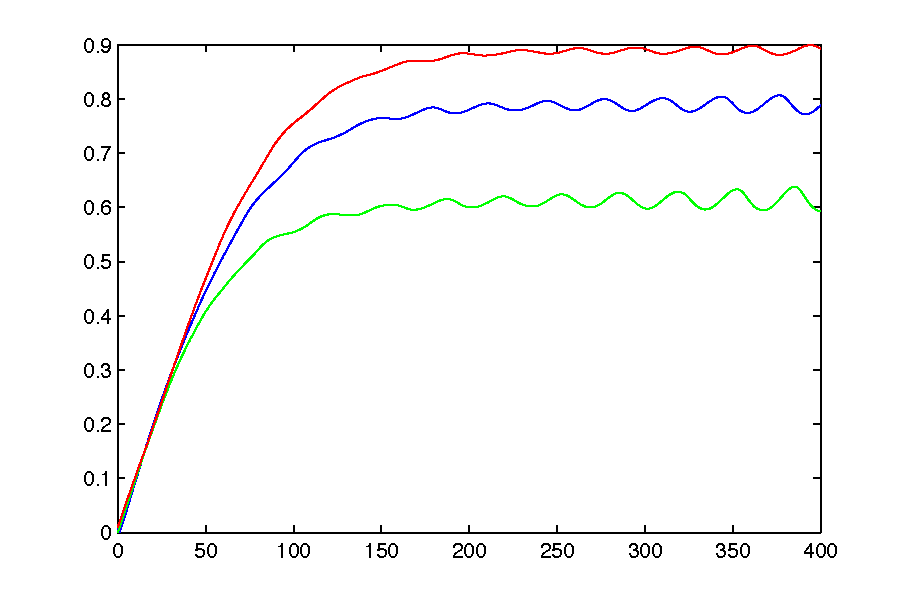
\includegraphics[width=0.7\textwidth]{straight-v-history}\\
& time~$t$
\end{tabular}
\caption{The mean velocity histories of the fluid flowing over the channel, shown in Figure~\ref{straight-channel}, at three random observed stations from the time~$t=0$ to~$t=400$. After the time~$t=200$, the slopes of the three curved are zeros in the horizontal direction, which indicate the fluid reach steady state. The ripples on these curves mean that small roll waves occur on the free surface.}
\label{straight-v-history}
\end{figure}%

\begin{figure}
\centering
\begin{tabular}{c@{}c}
\rotatebox{90}{\hspace{9ex}velocity~$\uu$} &
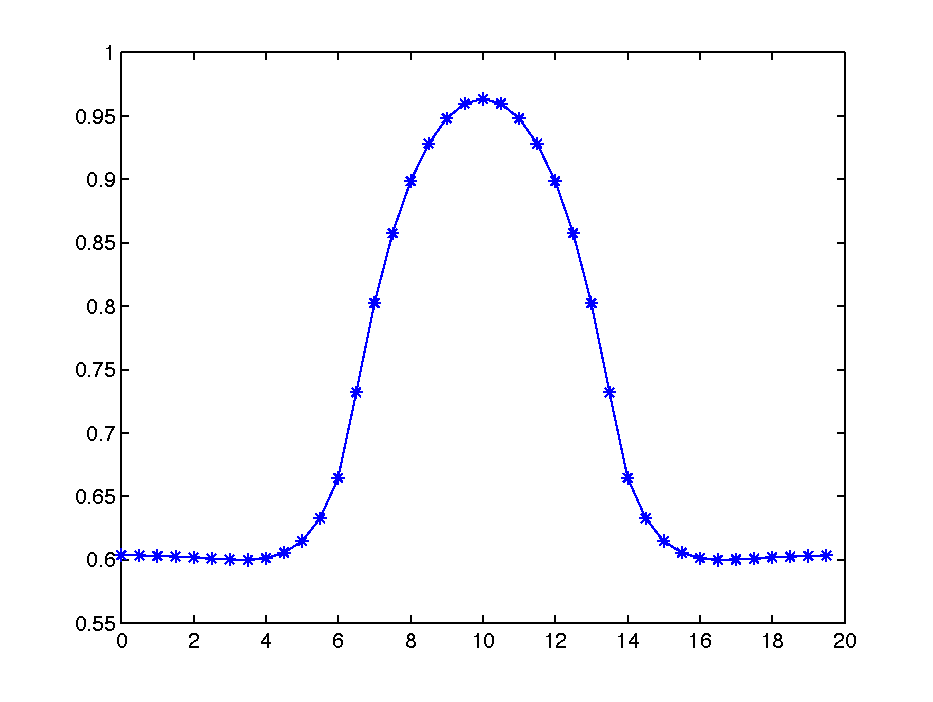
\includegraphics[width=0.7\textwidth]{straight-velocity-u}\\
& cross-section~$y$
\end{tabular}
\caption{Plot of the mean lateral velocity~$\uu$ in the cross-section at the point~$x=20$ and the time~$t=400$. The channel is nine times as deep in the middle as in the surrounding shallow regions, and the mean lateral velocity is one and a half times as fast in the middle as in the shallow regions.}
\label{straight-velocity-u}
\end{figure}%

\begin{figure}
\centering
\begin{tabular}{c@{}c}
\rotatebox{90}{\hspace{10ex}velocity~$\vv$} &
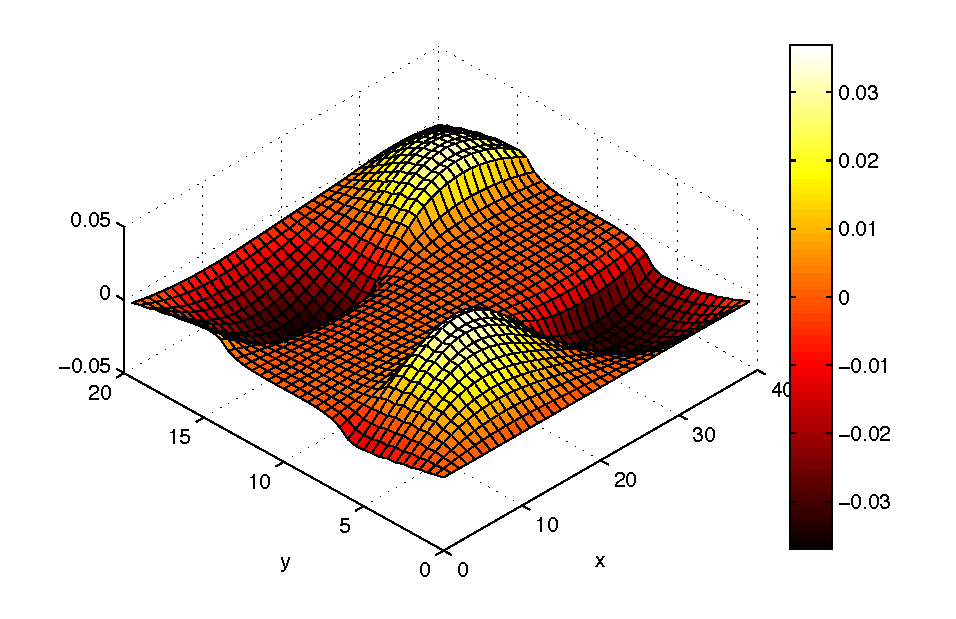
\includegraphics[width=0.7\textwidth]{straight-velocity-v}
\end{tabular}
\caption{The surf of the mean velocity~$\vv$ at time~$t=400$. The humps and dips indicate travelling vortices on the shear near the interactions between the channel and shallow regions.}
\label{straight-velocity-v}
\end{figure}%

\begin{figure}
\centering
\begin{tabular}{c@{}c}
\rotatebox{90}{\hspace{9ex}free surface} &
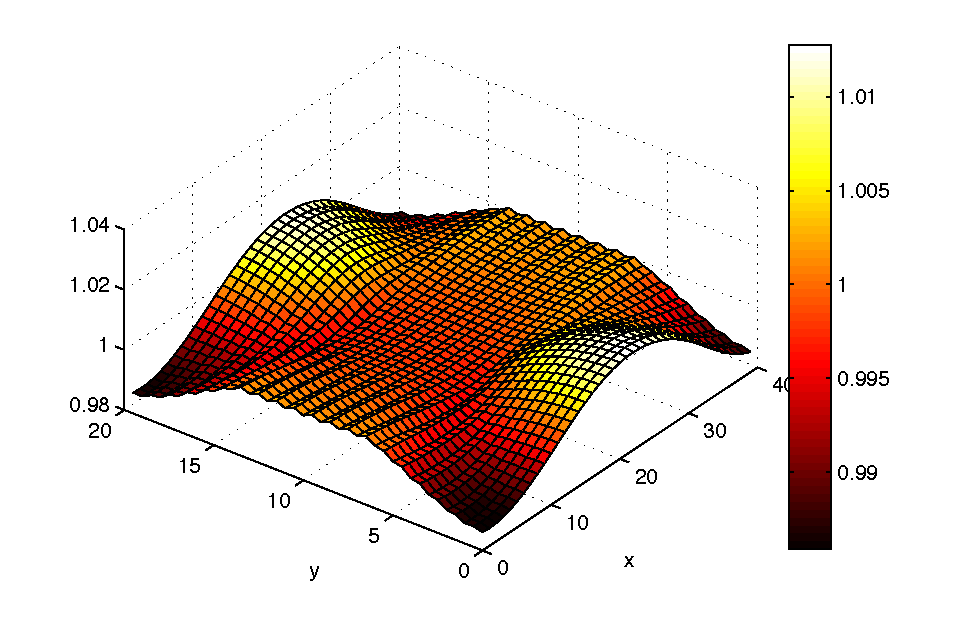
\includegraphics[width=0.7\textwidth]{straight-surface}
\end{tabular}
\caption{The simulation of free surface of the fluid at time~$t=400$. The relevant parameters are defined in Figure~\ref{straight-channel}. Big waves occur over the shallow regions and small waves are generated over the open channel. The small saw ripples in the cross-section are due to the numerical errors. }
\label{straight-surface}
\end{figure}%

\section{Modelling flows over meandering channels}
\label{sec-meander}

\begin{figure}
\centering
\begin{tabular}{c@{}c}
\rotatebox{90}{\hspace{16ex}$y$} &
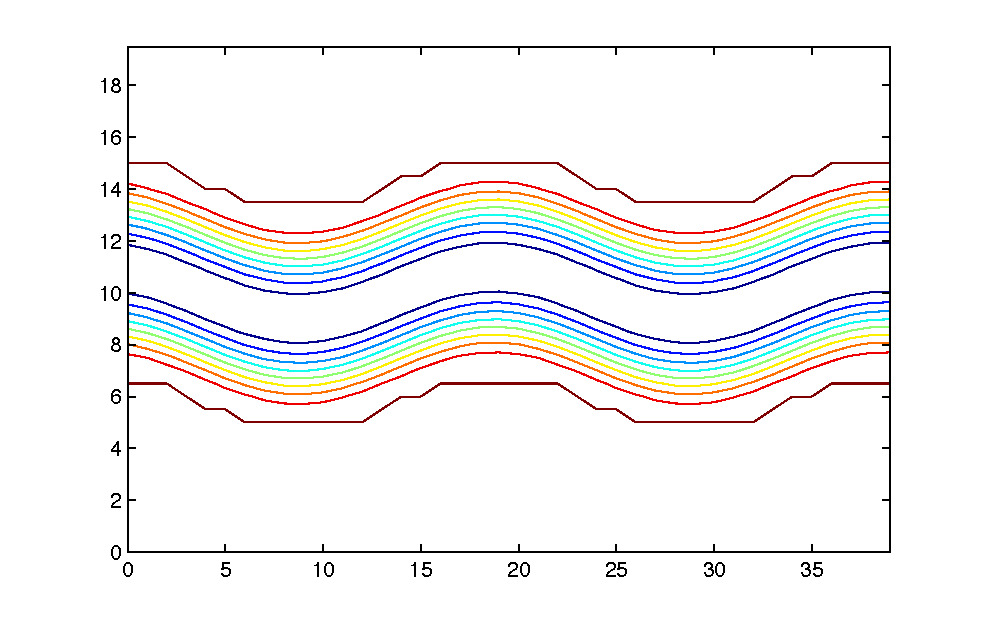
\includegraphics[width=0.7\textwidth]{meander-channel}\\
&~$x$
\end{tabular}
\caption{Contour of the meandering open channel. The channel locates around~$y=10$. The width and the maximum depth of the channel are~$8$ and~$0.9$, respectively. The parameters~$\kappa_1=1$ and~$\kappa_2=2\pi/L_x$ in equation~\eqref{bed:meander}, where~$L_x=40$ is the considered length in the~$x$ direction. The slope of the channel in the~$x$ direction is~$\theta=0.01$. Assume the still water level is~$1$, and thus the depth of the shallow regions is~$0.1$.}
\label{meander-channel}
\end{figure}%

This part describes the simulations of turbulent fluid flowing over a slightly sloped ground with a meandering open channel, shown in Figure~\ref{meander-channel}. The simulations are compared with the numerical results of~\cite{Liu2009} and~\cite{Demuren1993} who calculated the two and three dimensional turbulence flows in curved and meandering channels by a lattice Boltzmann model and a finite volume numerical model, respectively.

Create a Cartesian coordinate system~$(x,y,z)$. Consider nondimensionalised fluid depth~$h(x,y,t)$ and mean lateral velocities $\uu(x,y,t)$ in the~$x$ direction and~$\vv(x,y,t)$ in the~$y$ direction. Describe the meandering open channel~$b(x,y)$ by
\begin{align}&
b(x,y)=B\left\{1-\left[1-\left(\frac{y-\kappa_1\cos(\kappa_2x)-\alpha}{\beta}\right)^2\right]^2\right\}\,,\label{bed:meander}
\end{align}
where the parameter~$\kappa_1$ and~$\kappa_2$ determine the curvature of the meandering channel, and the parameters~$\alpha, \beta$ and~$B$ are defined as in equation~\eqref{bed:straight}.

Simulate the turbulent flow over such channel, shown in Figure~\ref{meander-channel}, by the equations~\eqref{smag:h}$-$\eqref{smag:v} with periodic boundary conditions in both~$x$ and~$y$ directions for both the flow and channel. Initially, consider the water of a constant depth~$h=1-b$ is still and impose a small noise to the zero mean lateral velocity~$\uu$ in the simulations. Figure~\ref{meander-v-history} exhibits the histories of the mean velocity~$\sqrt{\uu^2+\vv^2}$ of the fluid flowing over the channel, shown in Figure~\ref{meander-channel}, at three random observed stations from the time~$t=0$ to~$t=800$. No growing the mean velocity after the time~$t=500$ confirms that the simulations have converged to a steady state.

Simulations in Figure~\ref{meander-velocity} are the contours of the mean lateral velocities~$\uu$~(top) and~$\vv$~(bottom) at time~$t=800$. Black curves describe the shape of the meandering channel in the horizontal direction. The mean lateral velocity~$\uu$ reaches maximum at the bends and the mean lateral velocity~$\vv$ gets to maximum and minimum at the connection of the bends, which are consistent with the results of~\cite{Liu2009} who modelled the water in meandering channels with~$60^\circ$ and~$90^\circ$ consecutive bends and a width of~$0.3$\,m.~\cite{Demuren1993} calculated the depth and the depth-averaged longitudinal and transverse velocities of three dimensional flows in meandering channels with natural bed configuration by a finite volume numerical method. Simulations at~$15$ observed stations of the meandering channel indicate that the location of the maximum velocity shifts from the inner bank to the outer bank as the water flowing through the bends of the channel. Figure~\ref{meander-depth} and~\ref{meander-velocity-cross} show the plots of the depth~$h(x,y,t)$ and the mean lateral velocities~$\uu(x,y,t)$ and~$\vv(x,y,t)$ at the channel bends, which corresponds to the work of~\cite{Demuren1993}. The curves in Figure~\ref{meander-depth} and~\ref{meander-velocity-cross} are not very smooth because of the big spatial steps in the numerical computation. Reducing the spatial steps would reduce numerical errors and improve the accuracy.





\begin{figure}
\centering
\begin{tabular}{c@{}c}
\rotatebox{90}{\hspace{7ex}mean velocity~$\sqrt{\uu^2+\vv^2}$} &
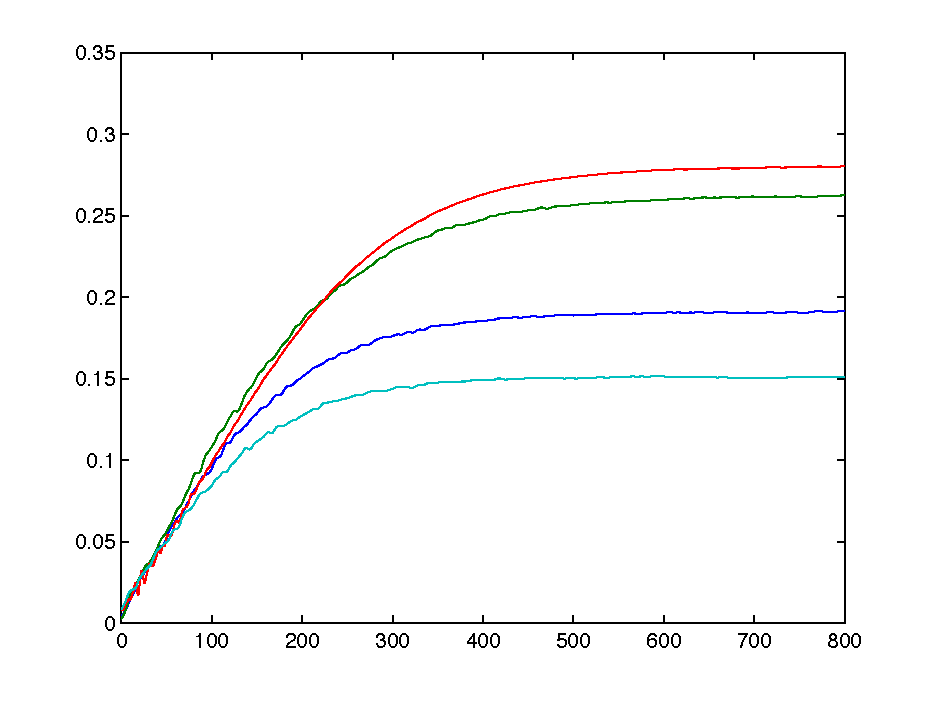
\includegraphics[width=0.7\textwidth]{meander-v-history}\\
& time~$t$
\end{tabular}
\caption{The mean velocity histories of the fluid flowing over the channel, shown in Figure~\ref{meander-channel}, at three random observed stations from the time~$t=0$ to~$t=800$. After the time~$t=500$, the slopes of the three curved are zeros in the horizontal direction, which support the fluid reach steady state.}
\label{meander-v-history}
\end{figure}%

\begin{figure}
\centering
\begin{tabular}{c@{}c}
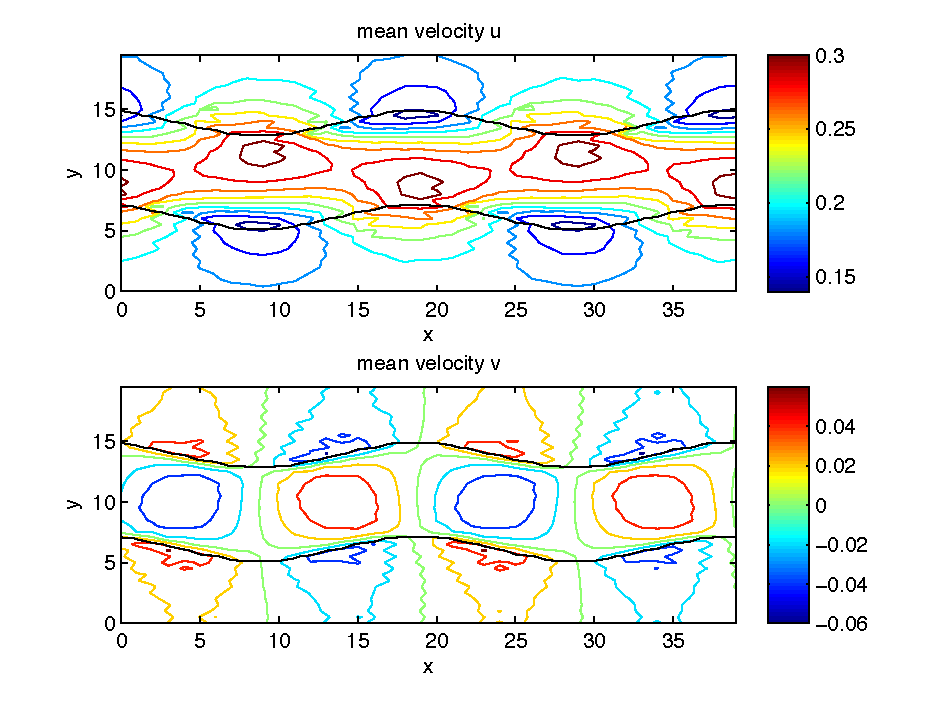
\includegraphics[width=0.7\textwidth]{meander-velocity}
\end{tabular}
\caption{Contours of the mean lateral velocities~$\uu$~(top) and~$\vv$~(bottom) at time~$t=800$. The black curves are the plots of the meandering channel. The lateral velocity~$\uu$ reaches maximum at the bends and the lateral velocity~$\vv$ gets to maximum and minimum at the connection of the bends.}
\label{meander-velocity}
\end{figure}%

\begin{figure}
\centering
\begin{tabular}{c@{}c}
\rotatebox{90}{\hspace{14ex}depth~$h$} &
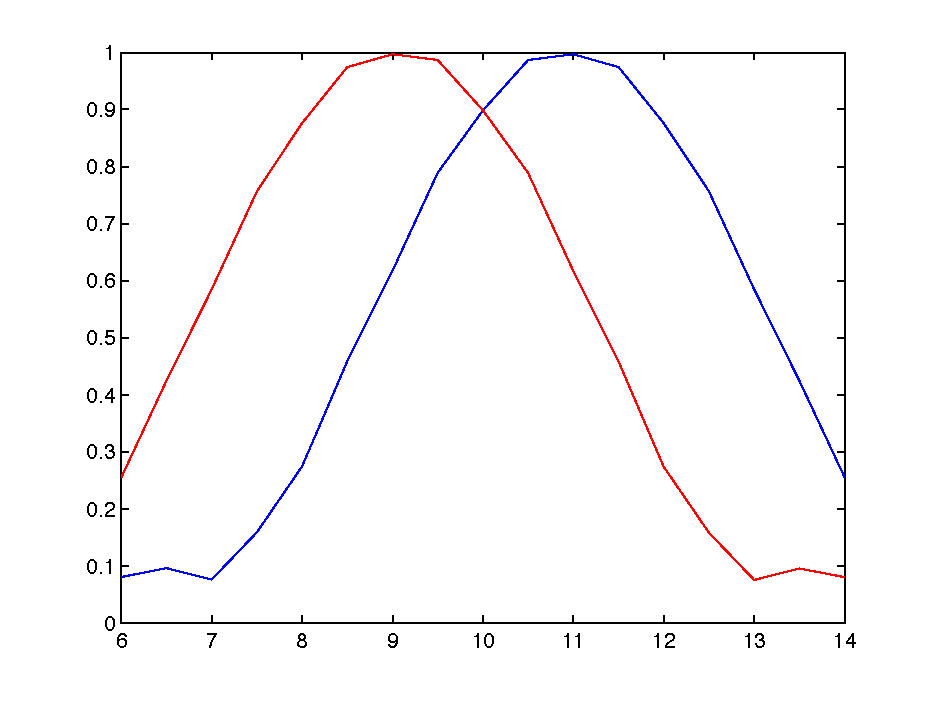
\includegraphics[width=0.7\textwidth]{meander-depth}\\
& channel cross-section
\end{tabular}
\caption{Plot of the fluid depth~$h(x,y,t)$ in the cross-section of the channel at stations~$x=10$~(red) and~$x=20$~(blue). The depth is big at the outer bank and small at the inner bank.}
\label{meander-depth}
\end{figure}%

\begin{figure}
\centering
\begin{tabular}{c@{}c}
\rotatebox{90}{\hspace{7ex}mean velocity~$\uu$ and~$\vv$} &
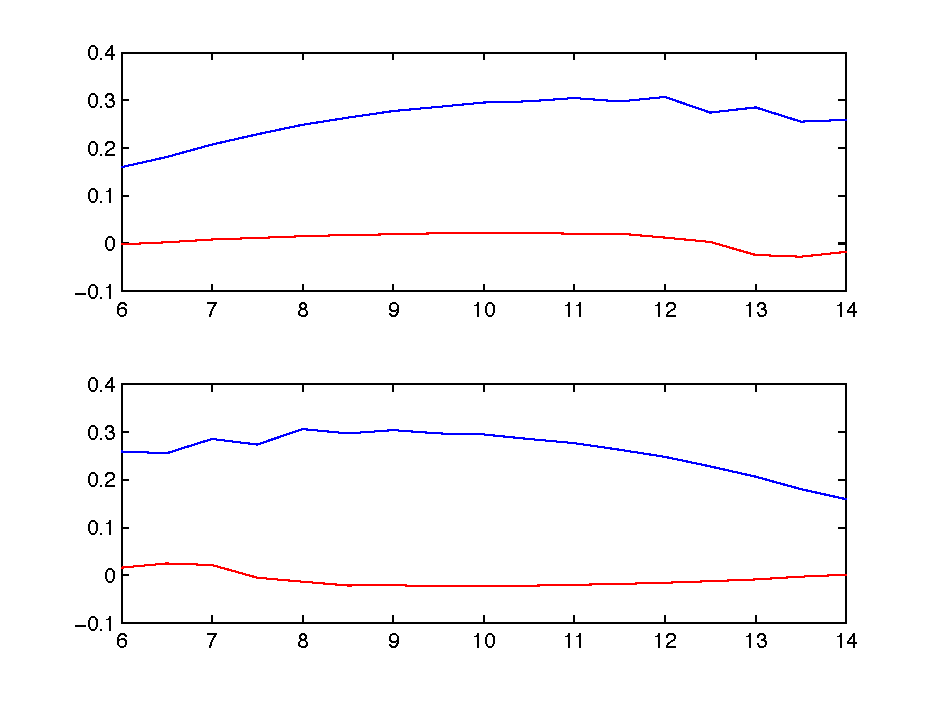
\includegraphics[width=0.7\textwidth]{meander-velocity-cross}\\
& channel cross-section\\
&blue:~$\uu(x,y,t)$\qquad red:~$\vv(x,y,t)$
\end{tabular}
\caption{Plots of the mean lateral velocities~$\uu(x,y,t)$~(blue) and~$\vv(x,y,t)$~(red) in the cross-section of the channel at stations~$x=10$~(top) and~$x=20$~(bottom). The location of the maximum mean velocity shifts from the inner bank to the outer bank as the fluid flowing through the bends.}
\label{meander-velocity-cross}
\end{figure}%



\section{Conclusion}

The proposed approach supporting by centre manifold theory describes the environmental turbulent fluids reliably. The flows in straight and meandering compound channel, as examples, are simulated by the new approach. The results correspond to the analysis and numerical simulations of the published work~\cite[e.g.]{Bousmar2002,Liu2009}. The equations~\eqref{smag:h}$-$\eqref{smag:v} account for the interactions between the vertical profiles and lateral spatial variations, and thus can be used to predict erosion and sand transport of the turbulent fluid in the further work.





\bibliographystyle{agsm}
\addcontentsline{toc}{section}{References}
\bibliography{turbulence}

\end{document}